\documentclass{article}
\usepackage{graphicx}
\usepackage[latin1]{inputenc}
\title{Tulha}
\author{FNU Tulha }
\date{October 2016}

\begin{document}

\maketitle

\section{Introduction}
\begin{equation}
f(x)= (1/((2\pi \sigma^2)^{0.5}))exp((-1/2)[(X-\mu )/\sigma]
\end{equation}

Since we have a continuous dataset we will first assume a Gaussian (normal) distribution for the training dataset.

\begin{equation}
f(x)= (1/((2\pi \sigma^2)^{0.5}))exp((-1/2)[(X-\mu )/6]    
\end{equation} 

But for one specific case:
\begin{equation}
p(x_{i}|y)=1/((2\pi \sigma_{y}^{2})^{0.5})e^{(-(x_{i}-\mu_{y} )^{2}/2\sigma _{y}^{2}})    
\end{equation}
    


So the features we would like to determine the posterior probability for, can be done using this.
The second thing we will assume is the independence of all these features and the probabilities of these features occuring given a specific class.


Training set
\begin{equation}
p(c|x_{i})=p(x_{i}|c)p(c)/p(x_{i})
\end{equation}

Where p($x_{i}$) is disregarded.
Where c is a class parameter c $\in{Yes, No}$ and Yes indicates 1 for Parkinson's disease and O for none. p($x_{1}$) is disregarded because it is the same for all posterior probabilities.

\begin{equation}
p(y=1|x=1)=p(x=1|y=1).p(y=1)    
\end{equation}

We were trying to determine:
\begin{equation}
p(y=1|x_{1},x_{2},....,x_{22})=\alpha 
\end{equation}
The above is for the 22 different features for this problem.
and

\begin{equation}
p(y=0|x_{1},x_{2},....,x_{22})=\beta
\end{equation}

If the ratio $\alpha$ / $\beta$ is greater than 1 then we label the datapoint as 1 ( meaning that for that configuration of features (x1,...x2) Parkisnson's disease would most likely be detected. Otherwise it won't.


\begin{figure}
\centering
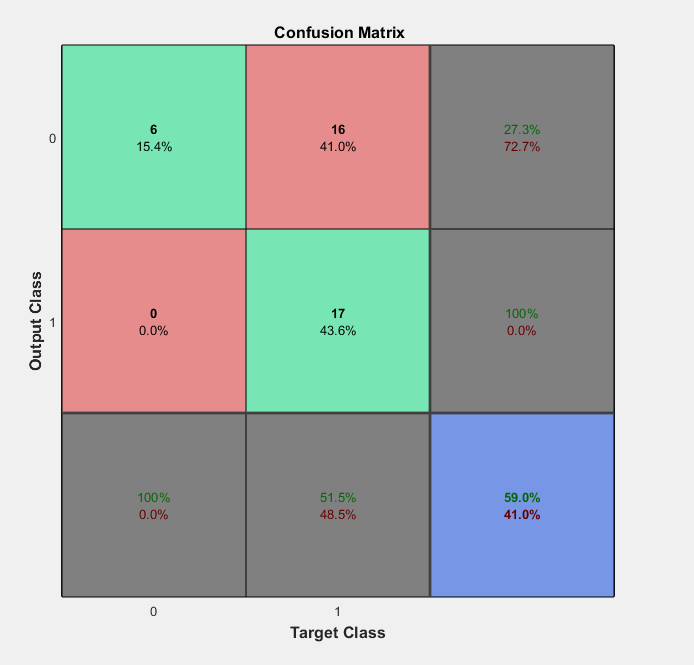
\includegraphics[width=0.7\linewidth, height=5.8cm]{confusiontask1.png}
\includegraphics[width=0.7\linewidth, height=5.8cm]{roctask1.png}


\renewcommand{\figure}{Fig.}

\caption{Results for task 1. }

\label{fig:1}
\end{figure}

The above files were generated using the algorithm for confusion matrix. Regarding the quality of the data analysis, since the assumption that all the feautures are independent can prove to be troublesome in some cases this may not be a very good data set analysis algorithm(naive bayes) in this case. Since the voice measurements may be dependant on other factors as well, this assumption will lead to less accurate results.
If the size of the training set is reduced, then the posterior probabilities for the test set will be least close to being accurate. The estimates for the mean and variance calculated by classifying the dataset into binary decisions(yes and no for the mean and standard deviation), it can be said that the estimates will get closer to inaccuracy as the size of the training set is reduced in this scenario. 

In the second problem we have to first divide the dataset into I's and 0's according to the labels that are present (training). $\sigma_{1}$,$\sigma _{0}$ will be evaluated according to this using the CO function of matlab. After this $\mu _{1}$ and $\mu_{0}$ will be evaluated too for the 4 features present.
The binary decision boundary equation. That was discussed in class will be used to label the test set.
\begin{equation}
p(w_{1}|x)/p(w_{2}|x)> 1 
then chose w_{1} (Both criteria have to be met)
p(x|w_{1})/p(x|w_{2})>  p(w_{2})/p(w_{1})    
\end{equation}


The resulting equation is:
\begin{equation}
x^{'}((\sigma_{0}^{-1})-(\sigma _{1}))x + 2((\sigma _{1}^{-1})\mu _{1} -(\sigma _{0}^{-1})\mu _{0})^{'}x+\mu _{0}^{'}\sigma _{0}^{-1}\mu _{0}-\mu _{1}^{'}\sum _{1}^{-1}\mu _{1}- log((\left |\sigma _{1}  \right |)/(\left |\sigma _{0} \right |) )- 2 log(p(w_{1})/p(w_{2}))>1    
\end{equation}
Please note that sigma here is actually the covariance.
\heading{Multivariate Gaussian Distribution}


\begin{equation*}
p(x)= (1/(2\pi)^{d/2}|\sigma |^{1/2})exp(-1/2(x-\mu)^{'}\sigma ^{-1}(x-\mu))
\end{equation*}

This equation was used to generate the probabilities of Yes cases and the probMatrix in the code file was given as input to the function. This generated a very accurate confusion matrix with few number of errors compared to naive bayes.
\end{document}








